\section{Challenges for Genomics} %  in the Age of Big Data
\begin{overview}
In this section, the main problems with contemporary genomics are considered. These problems must be solved to implement the concept of Genomics 2.0: the ubiquitous expansion and application of personal genomic technologies.
\end{overview}



\subsection{Low availability of genome analysis}

The costs for different types of genome analysis are listed in the Table~\ref{table:genomeanalysistypes} and, in general, starts from \$100. This price scale is extremely low relatively to the cost of genome reading 5 or 10 years ago\cite{Sboner2011}.

However, the price of sequencing and bioinformatic interpretation remains high enough that providing the general public with access to genomic analysis is difficult, especially in developing countries.


\begin{table}[H]
\caption{Genome analysis types.}
\label{table:genomeanalysistypes}

\textbf{DNA microarray} \newline
\begin{tabular}{r|p{11cm}} \hline
    \small\textbf{Description:} &
        \small analysis of 1-5 million pre-selected SNPs \\
    \small\textbf{Price range:}         & \small \$100-500 \\
    \small\textbf{Information amount}   & \small 0.033\% of full genome \\
    \small\textbf{Service providers}    & \small
     \href{https://www.23andme.com/}{23andMe},
     \href{https://www.ancestry.com/dna/}{AncestryDNA},
     \href{https://www.dnafit.com/}{DNAfit}.\\
\end{tabular}
\vskip0.2cm

\textbf{Genes panels} \newline
\begin{tabular}{r|p{11cm}} \hline
    \small\textbf{Price range:}         & \small \$100-2000 \\
    \small\textbf{Information amount}   & \small 0.001-1\% of full genome \\
    \small\textbf{Service providers}    & \small
     \href{https://www.pathway.com/}{Pathway Genomics},
     \href{http://www.cegat.de/en/}{CeGaT}.\\
\end{tabular}
\vskip0.2cm


\textbf{Exome sequencing} \newline
\begin{tabular}{r|p{11cm}} \hline
    \small\textbf{Description:} &
      \small Sequencing for the coding part of a genome (exome) \\
    \small\textbf{Price range:}         & \small \$250-3000 \\
    \small\textbf{Information amount}   & \small 2\% of full genome \\
    \small\textbf{Service providers}    & \small
     \href{https://www.bgi.com}{BGI},
     \href{http://www.cegat.de/en/}{CeGaT}.\\
\end{tabular}
\vskip0.2cm


\textbf{Whole Genome Sequencing} \newline
\begin{tabular}{r|p{11cm}} \hline
    \small\textbf{Price range:}         & \small \$600-10000 \\
    \small\textbf{Information amount}   & \small 80-98\% of full genome \\
    \small\textbf{Service providers}    & \small
     \href{https://www.bgi.com}{BGI},
     \href{https://www.fullgenomes.com/}{FullGenomes},
     \href{http://www.humanlongevity.com/}{Human Longevity}.\\
\end{tabular}
\vskip0.2cm

\parbox{\textwidth}{\it\small Note: actually, a part of a genome will not be sequenced. Its size depends on the sequencing depth and the details of sample preparation process. So the term “Whole Genome Sequencing” actually means obtaining the sequence of slightly more than 80\% of a genome.}

\end{table}

Obtaining a large amount of genomic information (sequences of genomes together with phenotypic characteristics) for residents of developing countries is extremely important from the perspective of obtaining the widest possible diversity of genomic information that, in turn, will significantly stimulate the development of the genomic big data market. Even in the mostly developed countries, less than 2\% of the population has undergone any genomic analysis (microarray, exome sequencing, or whole-genome sequencing).




\subsection[Privacy compromising as a price for participation]{%
  Privacy compromising as a price for participation in open biomedical investigations.}

Informed consent for the collection and processing of personal data is a key issue in every biomedical research study. Any project involving human genome studies starts with the collection of signatures from individuals attesting to the fact that they understand the consequences and agree with the terms of the research study. The form of such consent varies depending on the project and may include giving permission to use the data in future projects, the consequences of which can be unpredictable.


\href{http://www.personalgenomes.org/}{In the Personal Genome Project},  supervised by Harvard Medical School, participants voluntarily agree that their data and samples of their genetic material can be used multiple times and can be made available to other laboratories. Participants of this project are specifically informed that their identity could be de-anonymized and that their private data could become public. This project aims to ensure that genomic data from as many people as possible will be openly available to stimulate new research and development in the genomics industry. The authors of the project believe that if we do not provide open access to genomic data and information exchange, we are at risk of ending up with thousands of isolated, privately stored collections of genomic data (from pharmaceutical companies, genomic corporations, and scientific centers), but each of these separate databases will not contain sufficient data to enable breakthrough discoveries.

\subsection[Multicentral scientific and clinical studies]{%
  Conducting international multicentral scientific and clinical studies.}

To perform new research and development in the field of genomics, it is necessary to conduct scientific and clinical studies on large samples from various population groups. Currently, collecting genomic samples from individuals with various ethnic backgrounds is difficult, as special projects need to be created, expeditions undertaken, and permission obtained from local regulators.

Today, only one startup is attempting to address this problem
\url{https://www.dnasimple.org/} for a small fee and with the promise of anonymity.

\subsection[Biobanks storing materials from various individuals]{Creation of biobanks storing materials from various individuals}

Biobanks serve as mediators between the donors of biological materials (blood samples, bone marrow samples, etc.) and researchers by processing the materials obtained and storing them for future use. In general, biobanks are a key tool for the progress of personalized (precision) medicine and drug development. One of the most important functions of biobanks is the collection of donor material for future use, including blood, bone marrow, and even germ cells.

Currently, biobanks are actively being developed in many countries. However, there is the possibility that the most valuable samples will belong to the most financially secure biobanks, for example, biobanks belonging to large pharmaceutical companies, which will lead to unequal access to biobank material for different categories of researchers. Therefore, there is a need to create biobanks in as many countries and cities as possible up to the limit of individual bio-reservoirs for each individual.

\subsection[Adjustment of analytical software for widespread application]{%
  Processing: genome analysis rate is limited by its bioinformatic processing. Adjustment of analytical software for widespread application.}

Currently, the speed of obtaining genomic data using genome analysis technologies (sequencing) is high and outstrips the speed of processing these data. If we consider any large-scale scientific study of a large number of genomes, the experimental steps of obtaining genomic information account for no more than 20\% of the study duration, while data processing comprises a much greater part of the project. Here, data processing means the steps taken from obtaining raw sequencing data to interpreting results and searching for various associations.

Another problem with modern software is that genomic analysis software was made by scientists and for scientists and thus requires adjustments to be widely applicable among physicians and for general consumers. As genomic analyzers the size of a USB stick already exist, the use of a personal sequencer in the same manner as a personal computer can be considered not science fiction but, rather, realistic in the near future.

\subsection[Genomic data interpretation]{Genomic data interpretation: mathematical models of disease developing risks}

Various models and algorithms are used to rank the risks of developing diseases based on genetic data. The primary types of these models are based on the type of inheritance considered: monogenic, polygenic and multifactorial. Assessing the risks of developing multifactorial or complex diseases requires accounting for the influence and interference of many genes as well as environmental factors. For a more detailed description of the available methods for assessing the risks of complex diseases, see\cite{Kalf2014,nature:complex-disease-risk}.

To develop a new model for assessing the risk of developing a disease, it is necessary to involve a large number of scientists. It is also necessary to investigate many publications regarding the disease being analyzed, to identify its type of inheritance, to determine the polymorphisms and mutations contributing to the development of the disease, and to develop "genomic algebra," that is, a set of rules for risk estimation. When a model has been established and validated in silico, clinical studies must be conducted to assess its applicability. This approach is currently the most accurate, but it is expensive in terms of the amount of time and effort required.

\subsection[Genomic data interpretation]{Genomic data interpretation: machine learning application.}
The use of machine learning algorithms to assess the risks of multifactorial diseases is being extensively investigated, but thus far, due to the lack of a sufficient number of training samples, existing mathematical models developed by biological scientists outperform machine learning approaches.

However, machine learning is already being used to predict certain complex characteristics of the human body. An example is the appearance of prediction in the work of Craig Venter and colleagues. The essence of their work involved analyzing the genomes and approximately 30,000 facial data points from several thousand volunteers. Based on the data obtained, training samples for machine learning algorithms were built and dependencies between genomic traits and individual appearance were determined. Because of this work, machines have learned to accurately restore a person's appearance based on his or her genomic data\cite{wired.co.uk:longevitydiseases,Telenti18102016}.

The results of this project enable the prediction of the appearance of a criminal or of an unborn child during the early stages of pregnancy. By obtaining a blood sample from a pregnant woman and extracting fetal DNA from the blood, the appearance of an unborn child on his or her 18th birthday can be accurately predicted.

To implement this project, Craig Venter recruited one of the best machine learning specialists from Google, Franz Och, a star computer scientist known as the chief architect of Google Translate\cite{forbes:illumina-grail}.

Currently, machine learning is not widely used for diseases, as very large and correctly structured samples are needed for training. The creation of a comprehensive database of human genomes, as well as the availability of detailed questionnaires reflecting individuals’ health statuses, can spur the development of computational training in genomics and will result in highly predictive accuracy in determining the risk of disease development. At the same time, these data will be public and available to all users of the system, excluding the possibility of their monopolization. This availability is extremely important, as the concentration of large amounts of data in corporations’ databases will result in monopolies in the field of genomic machine learning.

\subsection{Secure storing of very large data}

Personal data security is very important; we all try to prevent the theft of credit card data, insurance information, banking account numbers, and medical information of any type. The theft of genomic information may seem unimportant for many people today. However, it can lead to very serious consequences that are difficult to predict, for example, the possibility that a portion of an individual’s genomic sequence could be synthesized and planted at the site of a crime or a terrorist act.

Current solutions for this problem involve encrypted storage on a central server, such as\cite{Sousa2017}, \url{https://www.pathway.com/}, \url{https://www.23andme.com/}, or \url{http://www.humanlongevity.com/}. This type of “closed” data storage is relatively safe, but it prohibits the possibility of sharing data and providing access to scientists from all over the world, which is a critically important condition for the development of modern genomic science.

Another problem associated with storage concerns the large size of a genome itself, and the exponential growth of the amount of genomic data available, as more and more individuals are subjected to genome sequencing. In one study \cite{10.1371/journal.pbio.1002195}, by 2025, the total volume of stored genomic data (given the size of a complete genome is 100 Gb) is predicted to reach 40 exabytes per year and genomic storage is predicted to become one of the largest consumers of storage and information processing capacities.

\begin{table}[H]
  \caption{Four domains of Big Data in 2025.}


\textbf{Astronomy} \newline
\begin{tabular}{r|p{13cm}} \hline
    \small\textbf{Acquisition}  & \small 25 zetta-bytes/year \\
    \small\textbf{Storage}      & \small 1 EB/year \\
    \small\textbf{Analysis}     & \small
      In situ data reduction; Real-time processing; Massive volumes;\\
    \small\textbf{Distribution} & \small
      Dedicated lines from antennae to server (600 TB/s) \\
\end{tabular}

\vskip0.2cm


\textbf{Twitter} \newline
\begin{tabular}{r|p{13cm}} \hline
    \small\textbf{Acquisition}  & \small 0.5-15 billion tweets/year  \\
    \small\textbf{Storage}      & \small 1-17 PB/year  \\
    \small\textbf{Analysis}     & \small
      Topic and sentiment mining; Мetadata analysis \\
    \small\textbf{Distribution} & \small Small units of distribution \\
\end{tabular}
\vskip0.2cm



\textbf{YouTube} \newline
\begin{tabular}{r|p{13cm}} \hline
    \small\textbf{Acquisition}  & \small 500-900 million hours/year   \\
    \small\textbf{Storage}      & \small 1-2 EB/year   \\
    \small\textbf{Analysis}     & \small Limited requirements \\
    \small\textbf{Distribution} & \small Major component of modern user’s bandwidth (10 MB/s) \\
\end{tabular}
\vskip0.2cm



\textbf{Genomics} \newline
\begin{tabular}{r|p{13cm}} \hline
    \small\textbf{Acquisition}  & \small  1 zetta-bases/year  \\
    \small\textbf{Storage}      & \small  2-40 EB/year \\
    \small\textbf{Analysis}     & \small Heterogeneous data and analysis;
      Variant calling, $\sim$ 2 trillion central processing unit (CPU) hours;
      All-pairs genome alignments,  $\sim$ 10,000 trillion CPU hours. \\
    \small\textbf{Distribution} & \small Many small (10 MB/s) and fewer massive (10 TB/s) data movement \\
\end{tabular}

\end{table}


\begin{figure}[]\centering
  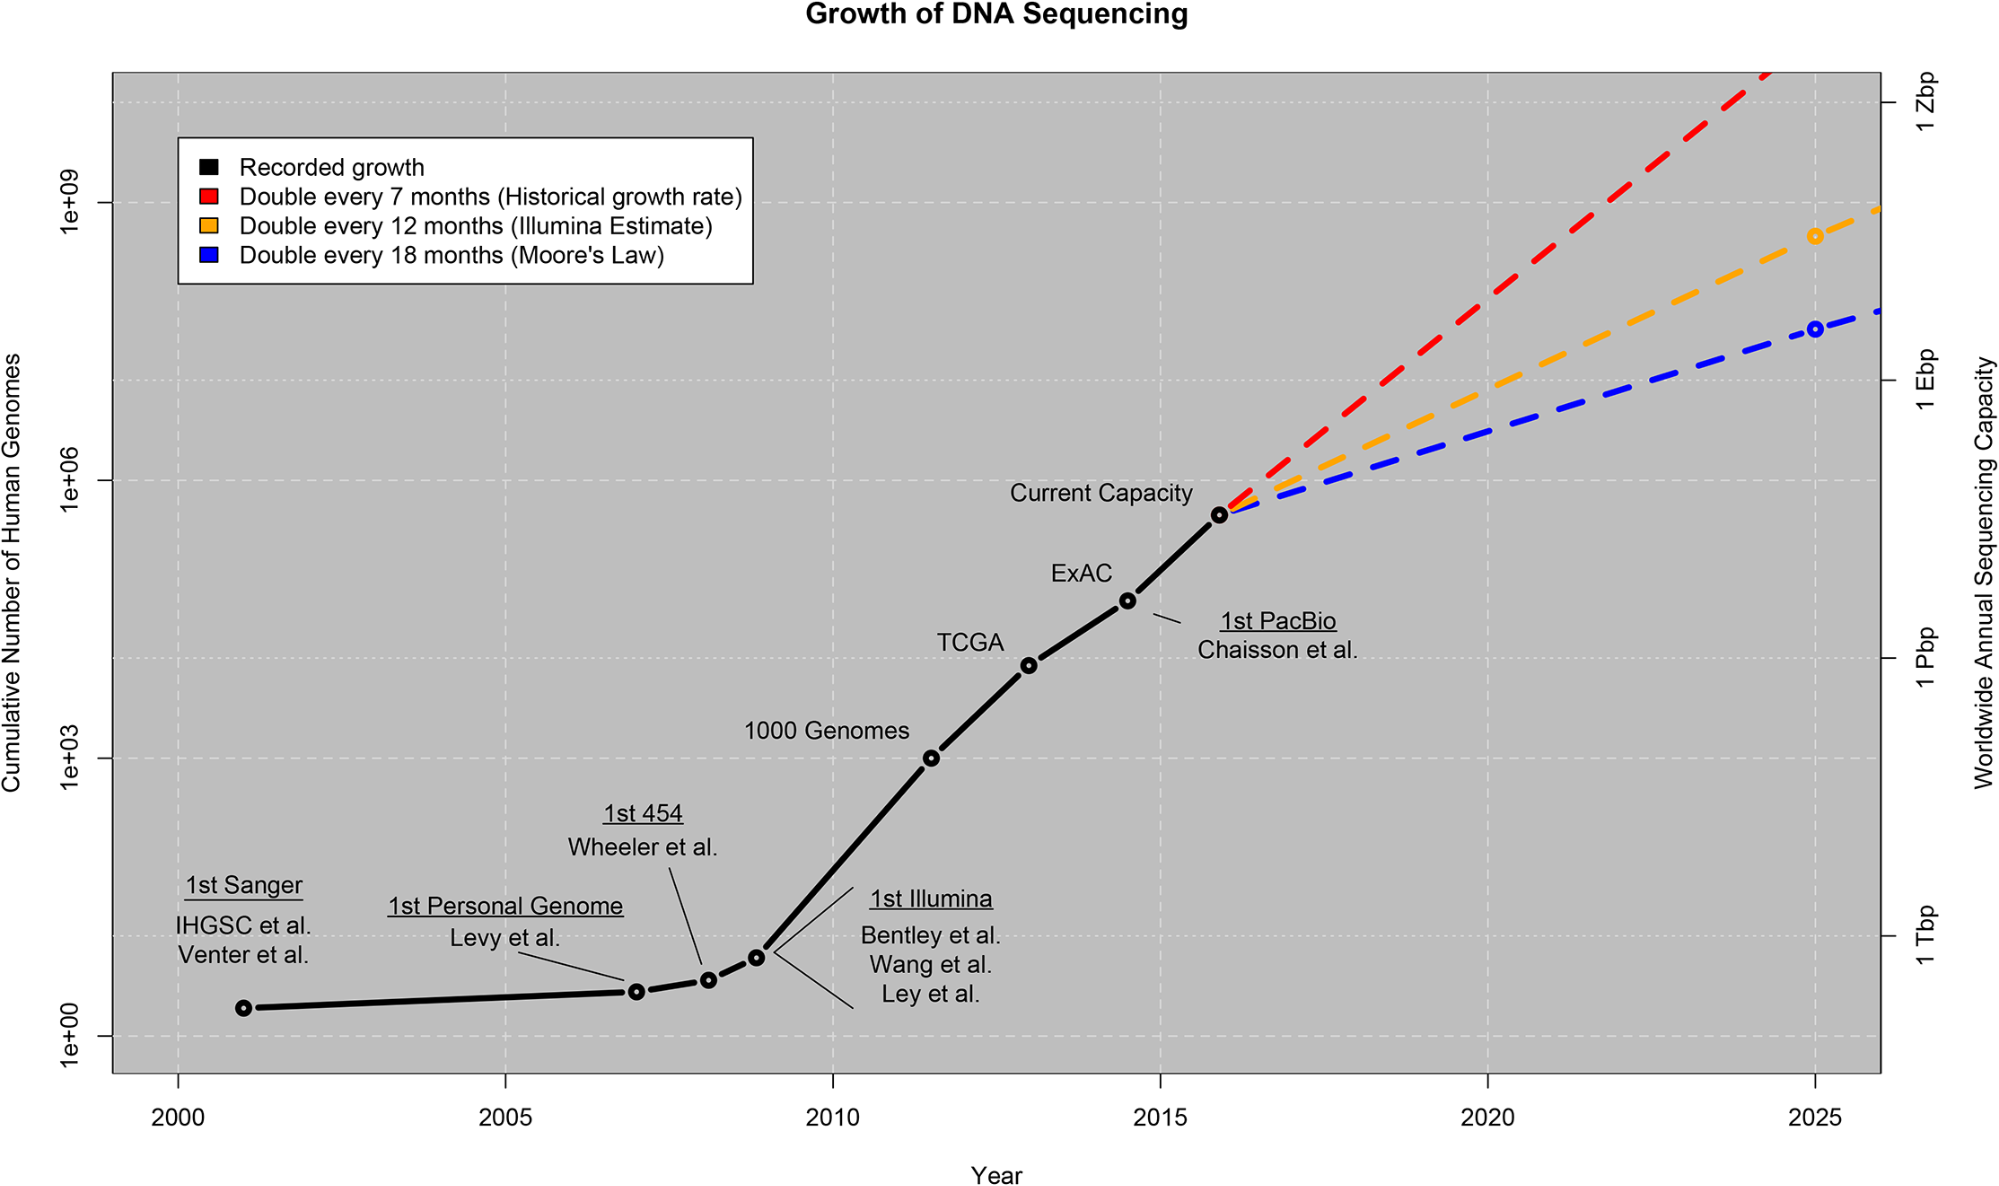
\includegraphics[width=\textwidth]{fig/Growth.png}
  \caption{Growth of DNA sequencing data. This plot shows the growth of DNA sequencing both in the total number of human genomes sequenced (left axis) and the worldwide annual sequencing capacity (right axis: Tera-basepairs (Tbp), Peta-basepairs (Pbp), Exa-basepairs (Ebp), and Zetta-basepairs (Zbp)). The values through 2015 are based on historical publication records with highlighted milestones in sequencing (first Sanger sequencing through the first PacBio human genome published) as well as three exemplary projects using large-scale sequencing: the 1000 Genomes Project, which aggregated hundreds of human genomes by 2012; The Cancer Genome Atlas (TCGA), which aggregated several thousand tumor/normal genome pairs; and the Exome Aggregation Consortium (ExAC), which aggregated over 60,000 human exomes. Many of the genomes sequenced to date represent whole exomes rather than whole genomes, but we expect this ratio to be increasingly biased toward whole genomes in the future. The values beyond 2015 represent our projections under three possible growth curves, as described in the main text.
Taken from \cite{10.1371/journal.pbio.1002195}.}
\end{figure}


\subsection[Database with continuously updated questionnaires]{%
  The need for common database with continuously updated questionnaires.}


At the same time, the lack of a public database implemented based on the concept of distributed storage and using open-source software could lead to the total domination of this market area by companies such as Google or Amazon due to their powerful servers\footnote{\url{https://cloud.google.com/genomics/}}. If corporations or pharmaceutical companies become monopolists in the field of genomic information, we will observe the slow and expensive development of medicine with current treatment approaches persisting instead of a future in which a disease could be prevented even before its development or at the earliest stages of its manifestation.


%[http://techonomy.com/2015/07/challenges-for-genomics-in-the-age-of-big-data/]

\subsection{The near future of genomics}

As a conclusion to this chapter, it is worth describing some hypothetical but technically feasible perspectives and dangers that could be faced by the genomic industry and society in general:
\begin{itemize}

  \item A reduction in the cost of genome analysis and the miniaturization of genomic sequencing devices %\url{http://www.bio-itworld.com/uploadedImages/Bio-IT_World/Top_Headlines/2014/12-Dec/MinION%20close%20up.jpg}
    down to the level of cell phone plug-ins;
  \item The explosive growth of genomic data and its storage and the emergence of “genomic hackers” and privacy issues (protecting data);
  \item The blanket distribution of genomic medicine and telehealth;
  \item Changes to the food industry involving the implementation of personalized nutrition based on genomes;
  \item The development of personalized drug therapy;
  \item Dating based on genomic compatibility;
  \item Personality identification using genomic information, including the ability to make payments and obtain services;
  \item An increase in the average lifespan in all countries, the extension of active longevity, and a strong bias toward senior populations, late pregnancies, and decreasing birthrates;
  \item The development of genome-editing technologies;
  \item Appearance design for future children and other developments that are difficult to imagine. For example, the technical possibility of selecting healthy children and determining their future appearance both at the embryo stage and by obtaining fetal DNA from a pregnant woman’s blood already exists \cite{wired.co.uk:longevitydiseases}.
\end{itemize}
